


Arousal post-Experiemnt:

\begin{figure}
  \centering
  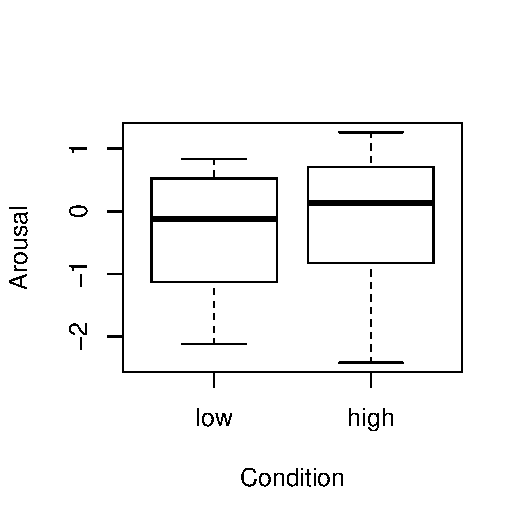
\includegraphics[width=0.5\linewidth,keepaspectratio] {images/arousalFactorPreBoxPlot-1}
  \caption{Athlete arousal prior to experiment, by condition}
        \label{fig:arousalFactorPreBoxPlot}
    \end{figure}

\begin{figure}
  \centering
      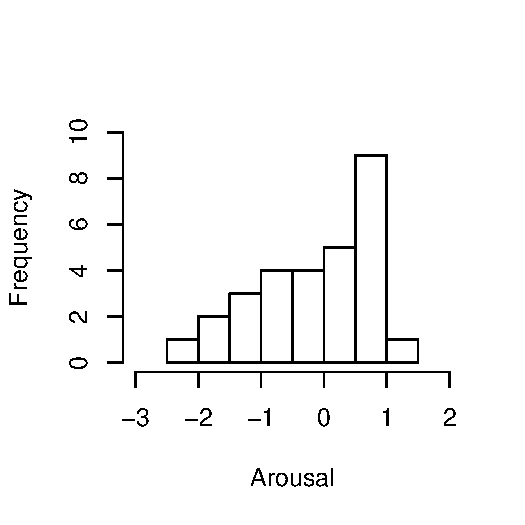
\includegraphics[width=0.5\linewidth,keepaspectratio] {images/histArousalFactorPreHigh-1}
      \caption{Histogram of athlete arousal prior to experiment (high difficulty condition)}
        \label{fig:histArousalFactorPreHigh}
    \end{figure}

\begin{figure}
  \centering
  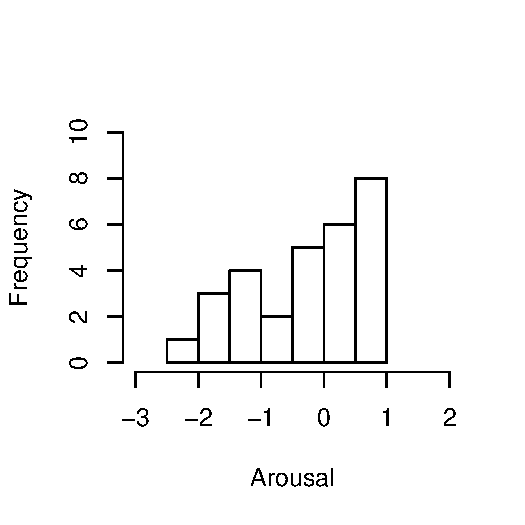
\includegraphics[width=0.5\linewidth,keepaspectratio] {images/histArousalFactorPreLow-1}
      \caption{Histogram of athlete arousal prior to experiment (low difficulty condition)}
  \caption{title}
    \label{fig:histArousalFactorPreLow}
\end{figure}














PRE-POST experiment results:

Histograms showing distribution of change variables:

"groupPerfChangeHist.pdf"
"indPerfChangeHist.pdf"
"groupClickChangeHist.pdf
"groupBondingChangeHist.pdf"
"teamBondingChangeHist.pdf"



Assumptions

~\ref{fig:M1PrePostAssumptions}


~\ref{fig:M2PrePostAssumptions}
